\begin{question}
	A clock is broken. It has only one hand which moves every hour either clockwise with probability 1/2 or counter-clockwise with probability 1/2 (the numbers are from 0 to 11 and the hand moves by one full hour when it moves). Assume it starts at 0. What is the probability that it reaches 7 before coming back to 0 for the first time?
\end{question}
\begin{ans}
	First, let's draw the graph representing the state space of the random variable of interest.
	\begin{center}
		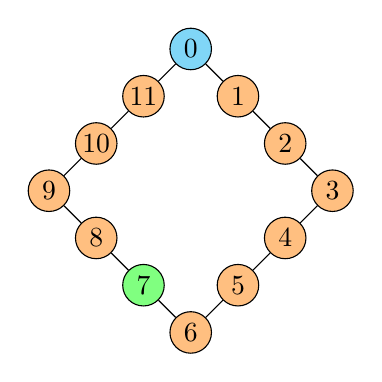
\begin{tikzpicture}[scale=0.6, every node/.style={circle, draw}]
			\tikzstyle{every node}=[circle, draw, fill=orange!50,
			inner sep=0pt, minimum width=15pt]
			
			
			\node[fill=cyan!50] (n0) at (0,3) {0};
			\node (n1) at (1,2) {1};
			\node (n2) at (2,1) {2};
			\node (n3) at (3,0) {3};
			\node (n4) at (2,-1) {4};
			\node (n5) at (1,-2) {5};
			\node (n6) at (0,-3) {6};
			
			\node (n11) at (-1,2) {11};
			\node (n10) at (-2,1) {10};
			\node (n9) at (-3,0) {9};
			\node (n8) at (-2,-1) {8};
			\node[fill=green!50] (n7) at (-1,-2) {7};
			
		
			\draw (n0) -- (n1);
			\draw (n1) -- (n2);
			\draw (n2) -- (n3);
			\draw (n3) -- (n4);
			\draw (n4) -- (n5);
			\draw (n5) -- (n6);
			\draw (n6) -- (n7);
			\draw (n7) -- (n8);
			\draw (n8) -- (n9);
			\draw (n9) -- (n10);
			\draw (n10) -- (n11);
			\draw (n11) -- (n0);
			
		\end{tikzpicture}
	\end{center}
	
	Define the event $B$ be $B = \set{T^+_0 > T_7}$. We are interested in finding $\prob_0(B)$. Now we can perform the first step argument as follows
	\[ p_0 = \frac{1}{2}(p_1 + p_{11}). \tag{3.1} \]
	Then we analyze each term in the right hand side of the equation above. For $p_1$ we have
	\[ \prob_1(B) = \underbrace{\prob_1(B|T_0>T_7)}_{1}\underbrace{\prob_1(T_0>T_7)}_{1/5} + \underbrace{\prob_1(B|T_0<T_7)}_{0}\underbrace{\prob_1(T_0<T_7)}_{6/7} = \frac{1}{5}. \]
	Note that $\prob_1(B|T_0>T_7)=1$ since it literally means the random walker reaches 7 before 0. Also $\prob_1(B|T_0<T_7)=0$ since the event $B$ is conditioned on reaching 0 before 7, which is clearly 0. The term $\prob_1(T_0>T_7)$ is computed using the Gambler's ruin analysis. Similarly, for the $p_{11}$ term we have
	\[ \prob_{11}(B) = \underbrace{\prob_{11}(B|T_0>T_7)}_{1}\underbrace{\prob_{11}(T_0>T_7)}_{1/7} + \underbrace{\prob_{11}(B|T_0<T_7)}_{0}\prob_{11}(T_0<T_7) = \frac{1}{7}. \]
	The rationale behind the values of the terms are the same as the ones discussed above. Now we can substitute everything in $(3.1)$
	\[ \boxed{p_0 = \frac{1}{2} (\frac{12}{35}) = \frac{6}{35}}. \]
	
\end{ans}